\documentclass{article}
\usepackage[utf8]{inputenc}
\usepackage{amsfonts}
\usepackage{amssymb}
\usepackage{amsmath}
\usepackage{amsthm}
\usepackage{enumitem}
\usepackage{bbold}
\usepackage{bm}
\usepackage{graphicx}
\usepackage{color}
\usepackage{hyperref}
\usepackage[margin=2.5cm]{geometry}
\begin{document}
\title{\Large{INFO8006: Project 2 - Report}}
\vspace{1cm}
\author{\small{\bf Pattraporn Joomnok - B6644932} \\
\small{\bf Chayapha Leksungnoen - B6735173} \\
\small{\bf Arrirat Mungyotklang - B6739485}}
\maketitle
\section{Bayes filter}
\begin{enumerate}[label=\alph*.,leftmargin=*]
\item Let $\mathcal F$ be the traversable cells, $X_t$ the ghost position,
$q_t$ Pacman's known position, and $d(x,q)=\|x-q\|_1$. For variance $v$,
$p=1/2$ and $n=\lfloor4v\rfloor$. The sensor is
\[E_t=d(X_t,q_t)+B_t-np,\qquad B_t\sim\operatorname{Binomial}(n,p).\]
For $k=e-d(x,q_t)+np$,
\[P(E_t=e\mid X_t=x,q_t)=
\begin{cases}\binom nk p^k(1-p)^{n-k},&k\in\{0,\ldots,n\},\\
0,&\text{otherwise}.\end{cases}\]
The conditional mean is $d(x,q_t)$ and actual variance is $n/4$.
At $v=1$, noise $(-2,-1,0,1,2)$ has probabilities $(1,4,6,4,1)/16$.
Odd $n$ gives half-integer noise; negative observations must not be
clipped. When $n=0$, the sensor is exact.
\item Let $N(x)=\{y\in\mathcal F:\|y-x\|_1=1\}$. For one free parameter
$\lambda\geq1$, assign weight $w_\lambda(y,x;q)=\lambda$ when
$d(y,q)\geq d(x,q)$, and $1$ otherwise. For $N(x)\ne\varnothing$,
\[T_\lambda(y\mid x,q)=
\begin{cases}w_\lambda(y,x;q)/\sum_{z\in N(x)}w_\lambda(z,x;q),&y\in N(x),\\
0,&\text{otherwise}.\end{cases}\]
Confused, afraid and scared correspond to $\lambda=1,2,8$.
Backtracking is allowed; there is no direction memory. Staying still
has zero probability if a neighbor exists. An isolated cell has a
self-transition of probability one.
\end{enumerate}
\section{Implementation}
\begin{enumerate}[label=\alph*.,leftmargin=*]
\item \textbf{\textit{Leave empty.}}
\end{enumerate}
\newpage
\section{Experiment}
\begin{enumerate}[label=\alph*.,leftmargin=*]
\item Uncertainty is Shannon entropy in bits,
$H(b_t)=-\sum_{x\in\mathcal F}b_t(x)\log_2 b_t(x)$, with $0\log0=0$.
Smaller values mean more concentrated beliefs. Eaten ghosts are excluded.
\item Quality is expected Manhattan distance to true position $x^*$,
$L(b_t,x^*)=\sum_x b_t(x)d(x,x^*)$. Smaller is better. Unlike entropy,
it penalizes belief mass far from truth. Ground truth is used for evaluation.
\item We ran 180 trials: two layouts, three policies, variances
$\{0.25,1,4\}$ and ten seeds (0--9), with one ghost and 200 observations
per trial. All trials reached 200 steps. Pacman uses the same random
walker throughout, reading ground truth to avoid collisions; the
filter does not. Results depend on this observation trajectory.
Curves show trial means with pointwise 95\% Student-$t$ intervals.
Bars and variance comparisons use one mean per trial over $t=100$--199;
time steps are not treated as independent trials.
\begin{center}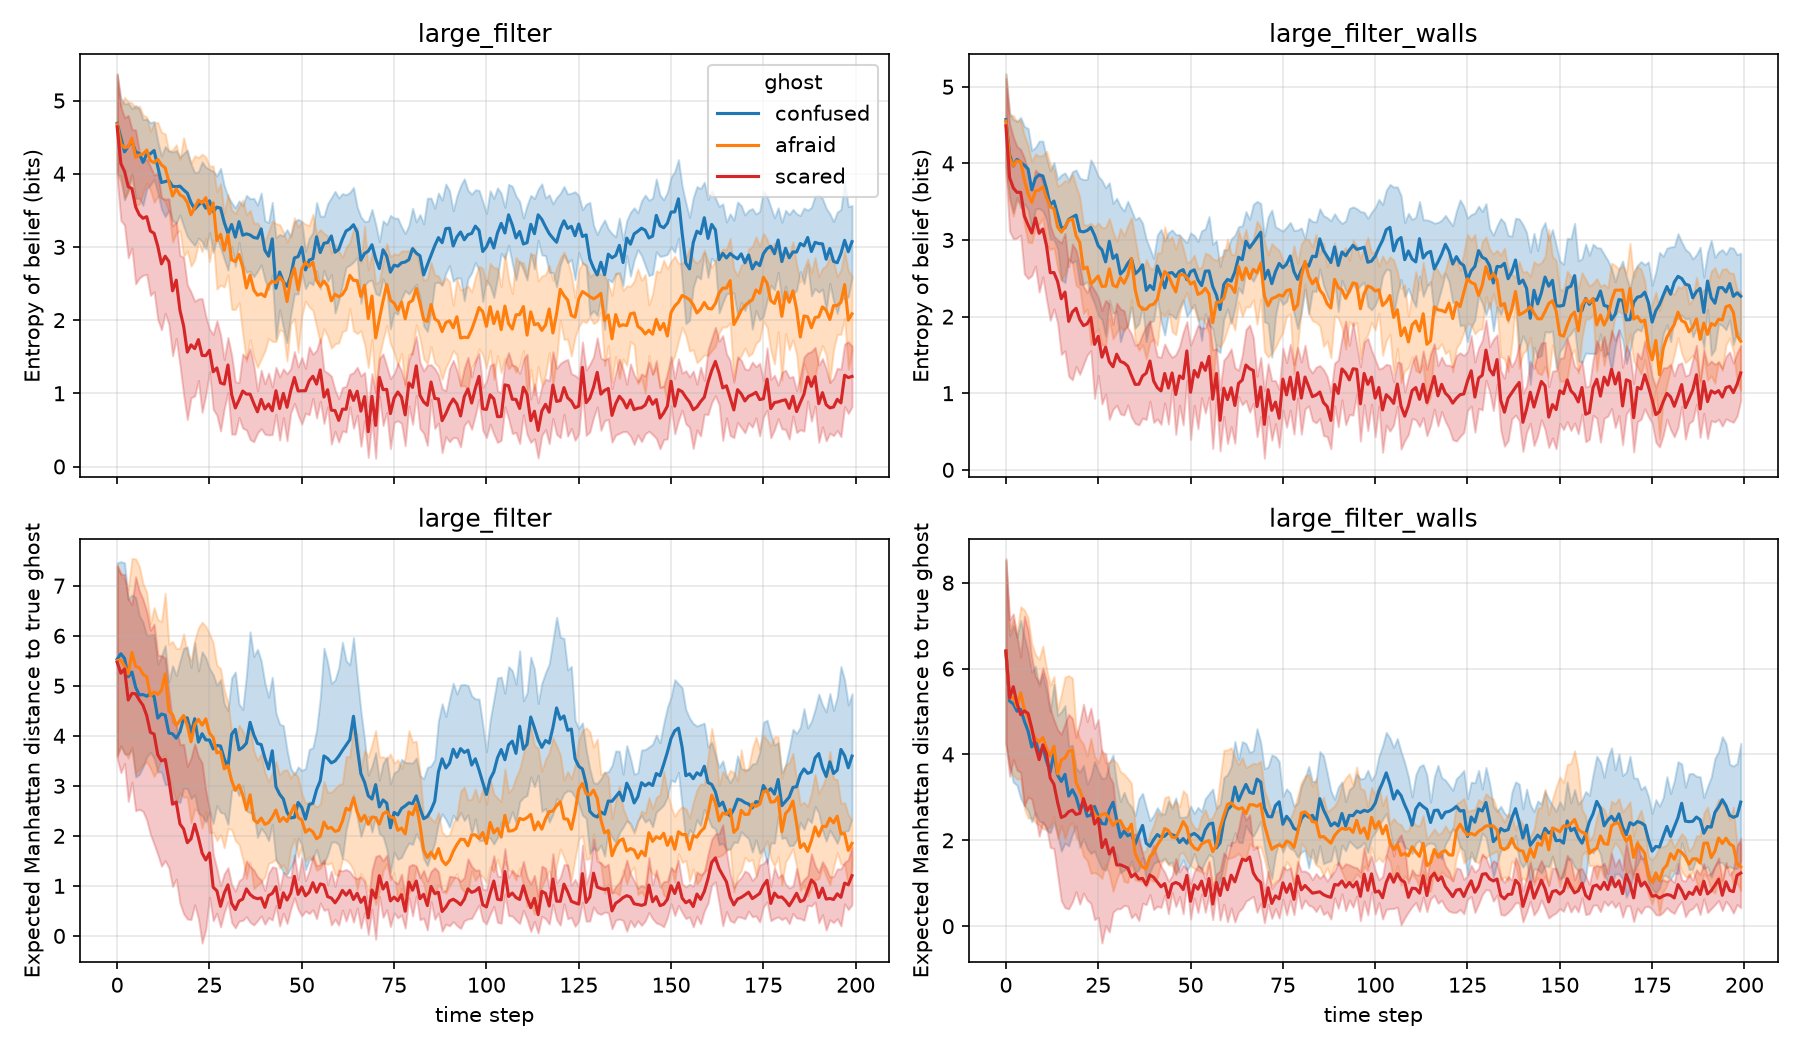
\includegraphics[width=\linewidth]{review_figs/curves_default_variance.png}
\\\small Figure 1: Default variance 1; shaded 95\% confidence intervals.
\end{center}
\newpage
\begin{center}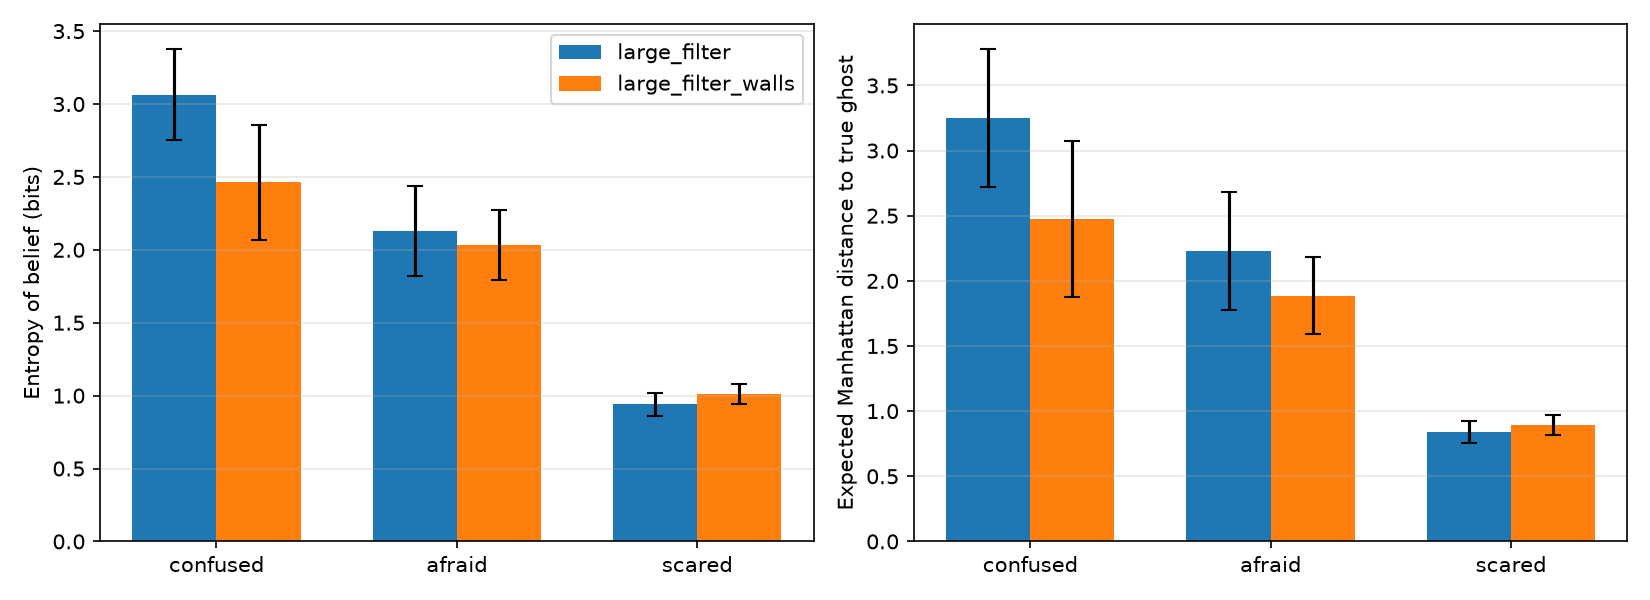
\includegraphics[width=\linewidth]{review_figs/steady_state_bars.png}
\\\small Figure 2: Late-window means and 95\% confidence intervals.
\end{center}
At variance 1, entropy/error on large\_filter are 3.063/3.248,
2.129/2.229 and 0.939/0.838 for confused/afraid/scared. On
large\_filter\_walls they are 2.462/2.473, 2.033/1.886 and 1.009/0.894.
Exact confidence intervals are in the accompanying summary.csv.

\textbf{Convergence:} for confused on large\_filter\_walls, comparing
$t=150$--199 against $t=100$--149 gives entropy changes
$-0.428\pm0.288$ bits at $v=1$ and $-0.262\pm0.195$ at $v=4$
(paired 95\% intervals). We extended these conditions to 1,000 steps
with the same ten seeds. All 20 extended trials reached 1,000 steps.
Comparing $t=750$--999 with $t=500$--749, entropy drift is
$-0.148\pm0.143$ bits at $v=1$ and $-0.167\pm0.117$ at $v=4$.
Some drift remains; we do not claim convergence.
Small drift or an interval containing zero does not prove
convergence. The ten-trial baseline remains a limitation.
\item With $a$ non-decreasing-distance and $b$ decreasing-distance
neighbors, escape probability is $\lambda a/(\lambda a+b)$.
For $a=b=1$, probabilities are $1/2,2/3,8/9$. If all neighbors belong
to one group, changing $\lambda$ has no effect. Dead ends can force
motion toward Pacman. At default variance, scared has lowest entropy
and error on both layouts, consistent with stronger escape constraints.
Walls lower means for confused/afraid but raise them slightly for
scared. Neither greater fear nor more walls guarantees improvement in
every setting, and differences in means alone do not establish significance.
\newpage
\item\begin{center}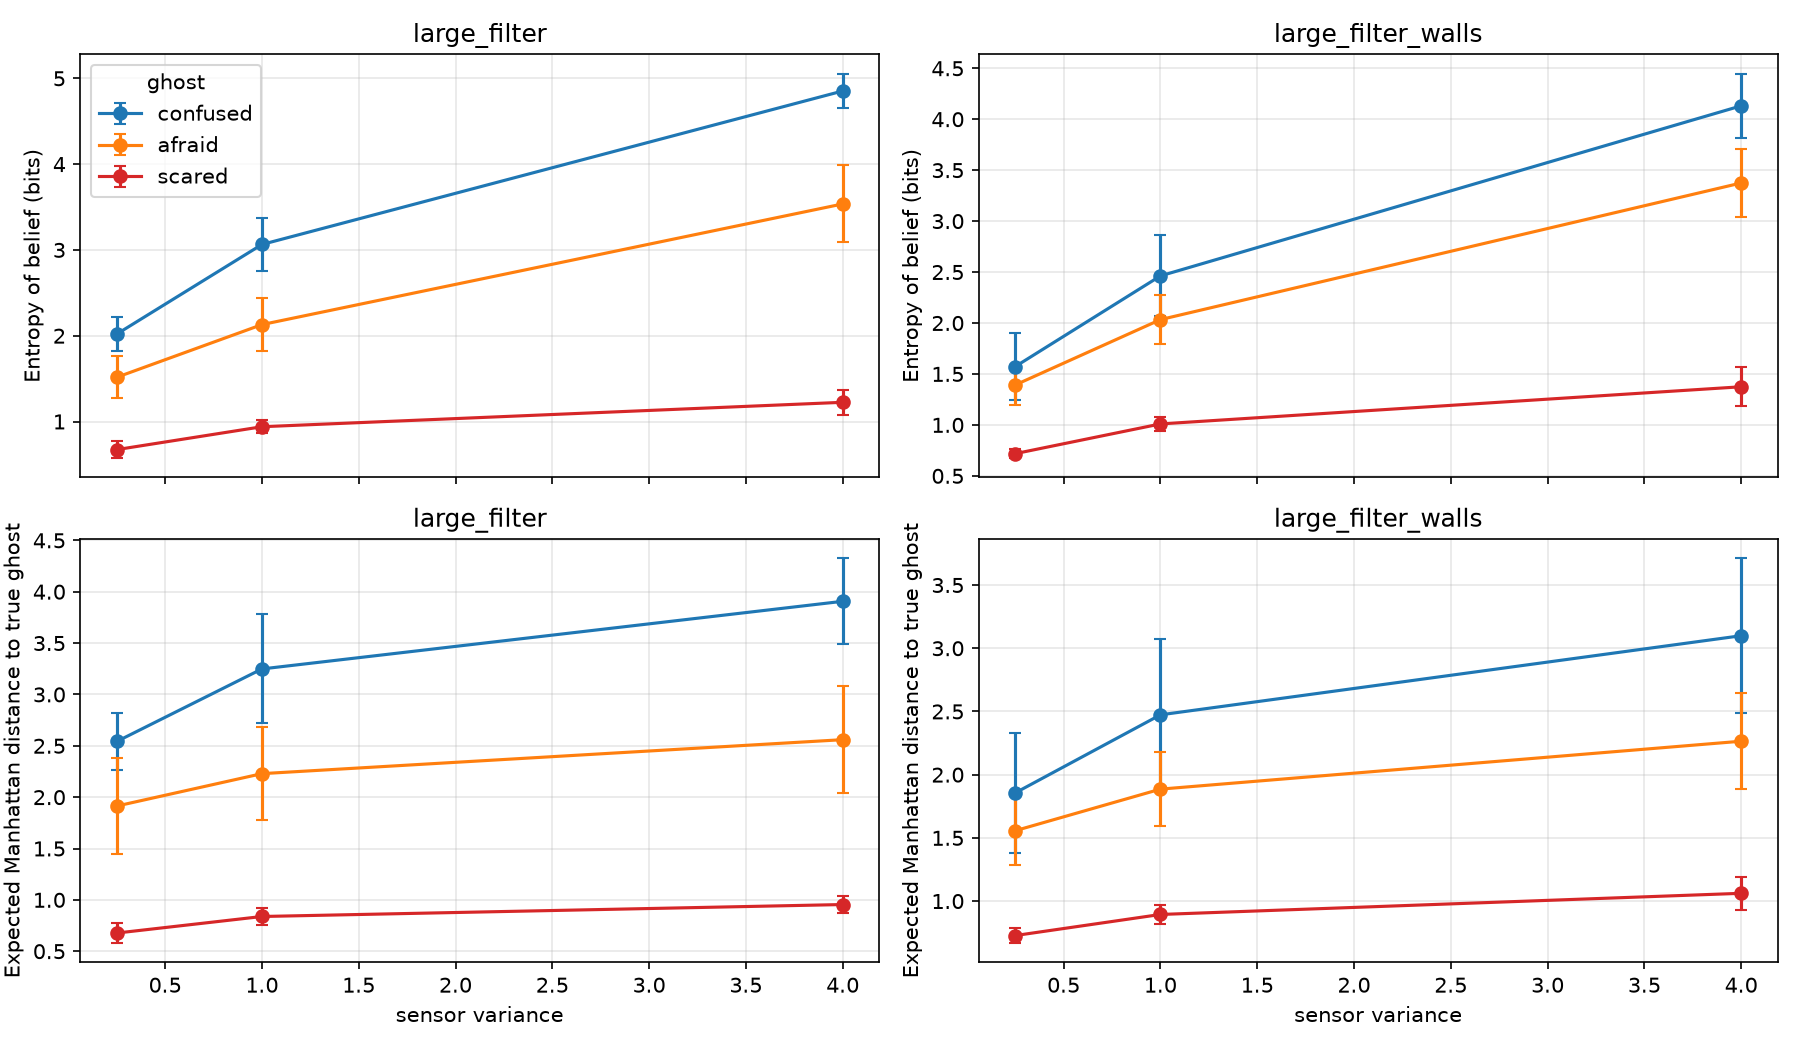
\includegraphics[width=\linewidth]{review_figs/variance_sweep.png}
\\\small Figure 3: Variance sweep, late-window means and 95\% intervals.
\end{center}
For every layout/policy pair, increasing variance from 0.25 to 1 to 4
increases mean entropy and error. Broader noise makes measurements
compatible with more cells, weakening correction. Scared remains
easier to localize in these trials. Chosen levels equal actual $n/4$;
other requested values may be rounded down.
\item Exclude zero-mass beliefs, choose the ghost with the smallest
expected Manhattan distance, then choose a legal non-STOP action
minimizing that expected distance at the successor. Break ties by
legal-action order. If no target or move exists, return STOP. Only
position, legal actions and beliefs are used. Greedy Manhattan distance
can oscillate around walls and does not guarantee capture.

Bonus smoke tests at seed 0, variance 1, one ghost and a 100-step cap
won all six pairs: 15/45/27 steps on large\_filter and 12/16/72 on
large\_filter\_walls. This is not a multi-seed success-rate estimate.
Three-ghost integration tests completed 60 steps for seeds 0 and 1.
\item \textbf{\textit{Leave empty.}}
\end{enumerate}
\end{document}
